\chapter{Experimental Results}
\label{chap:\currfilebase}

The data of both the fatigue testing machine and the CCD camera system have been recorded and stored. One can find an overview of all test data acquisition in \autoref{tab:specimen_overview}. The description of the used labelling system is located in \autoref{sec:specimen}.

\section{Stress over Strain Curves}
\label{sec:stress_strain_curves}

For the stress-strain curves both the measurement data of the fatigue test system and the footage of the CCD camera are used. The compressive stress of the specimen is assumed to be the force acting on the fatigue test system divided by the specimen cross-section at zero load:
\begin{align*}
    \sigma_c &= \frac{F_{c}}{S}, &S &= \frac{1}{3}\sum\limits_{i=2}^4 w_i\cdot t_i
\end{align*}
where $\sigma_c$ is the compressive stress, $F_c$ the compressive force measured by the fatigue test system, $S$ the mean cross section of the specimen and $w_i$, $t_i$ the width and thickness of said specimen, measured at position $i$.

The strain is assumed to be the mean of the local strains generated by DIC of the CCD camera footage:
\begin{align*}
    \varepsilon_{xx} &= \frac{1}{N}\sum\limits_{i\in\text{FOI}}\varepsilon_{xx,i}, &N &= \sum\limits_{i\in\text{FOI}}1
\end{align*}
\begin{align*}
    \text{FOI} &= \Bqty{i|p_{x,\min}\leq p_x(i)\leq p_{x,\max} \cap p_{y,\min}\leq p_y(i)\leq p_{y,\max}}
\end{align*}
where $\varepsilon_{xx}$ is the mean strain in compressive direction, $\varepsilon_{xx,i}$ the local strain in compressive direction at local point $p(i)=\pqty{p_x(i),p_y(i)}$, $\text{FOI}$ the field of interest, defined manually for each measurement by $p_{x,\min}$,$p_{y,\min}$,$p_{x,\max}$ and $p_{y,\max}$ and $N$ is the number of local strains inside the field of interest.

To avoid overlap of the FOI with the test fixture at high strains, resulting in a distortion of the strain mean, the dimension of the FOI in compressive direction was resized proportional to the displacement measured in the fatigue test machine. The stiffness of the press yoke was assumed to be high enough so that the FOI would not have a rigid body motion in compressive direction. The boundaries of the FOI thus remained constant with the exception of $p_{x,\min}$:
\begin{align*}
    p_{x,\min} &= p_{x,\min}(\Delta L)
\end{align*}
where $p_{x,\min}$ is the lower limit of the FOI in compressive direction and $\Delta L$ the displacement of the press piston from its initial position.

The stress-strain curve of the test 90A1 is shown in \autoref{fig:90A1_Stress_over_Strain}. For further test results one can consult \autoref{sec:apx_stress_strain}.

\begin{figure}[!ht]
    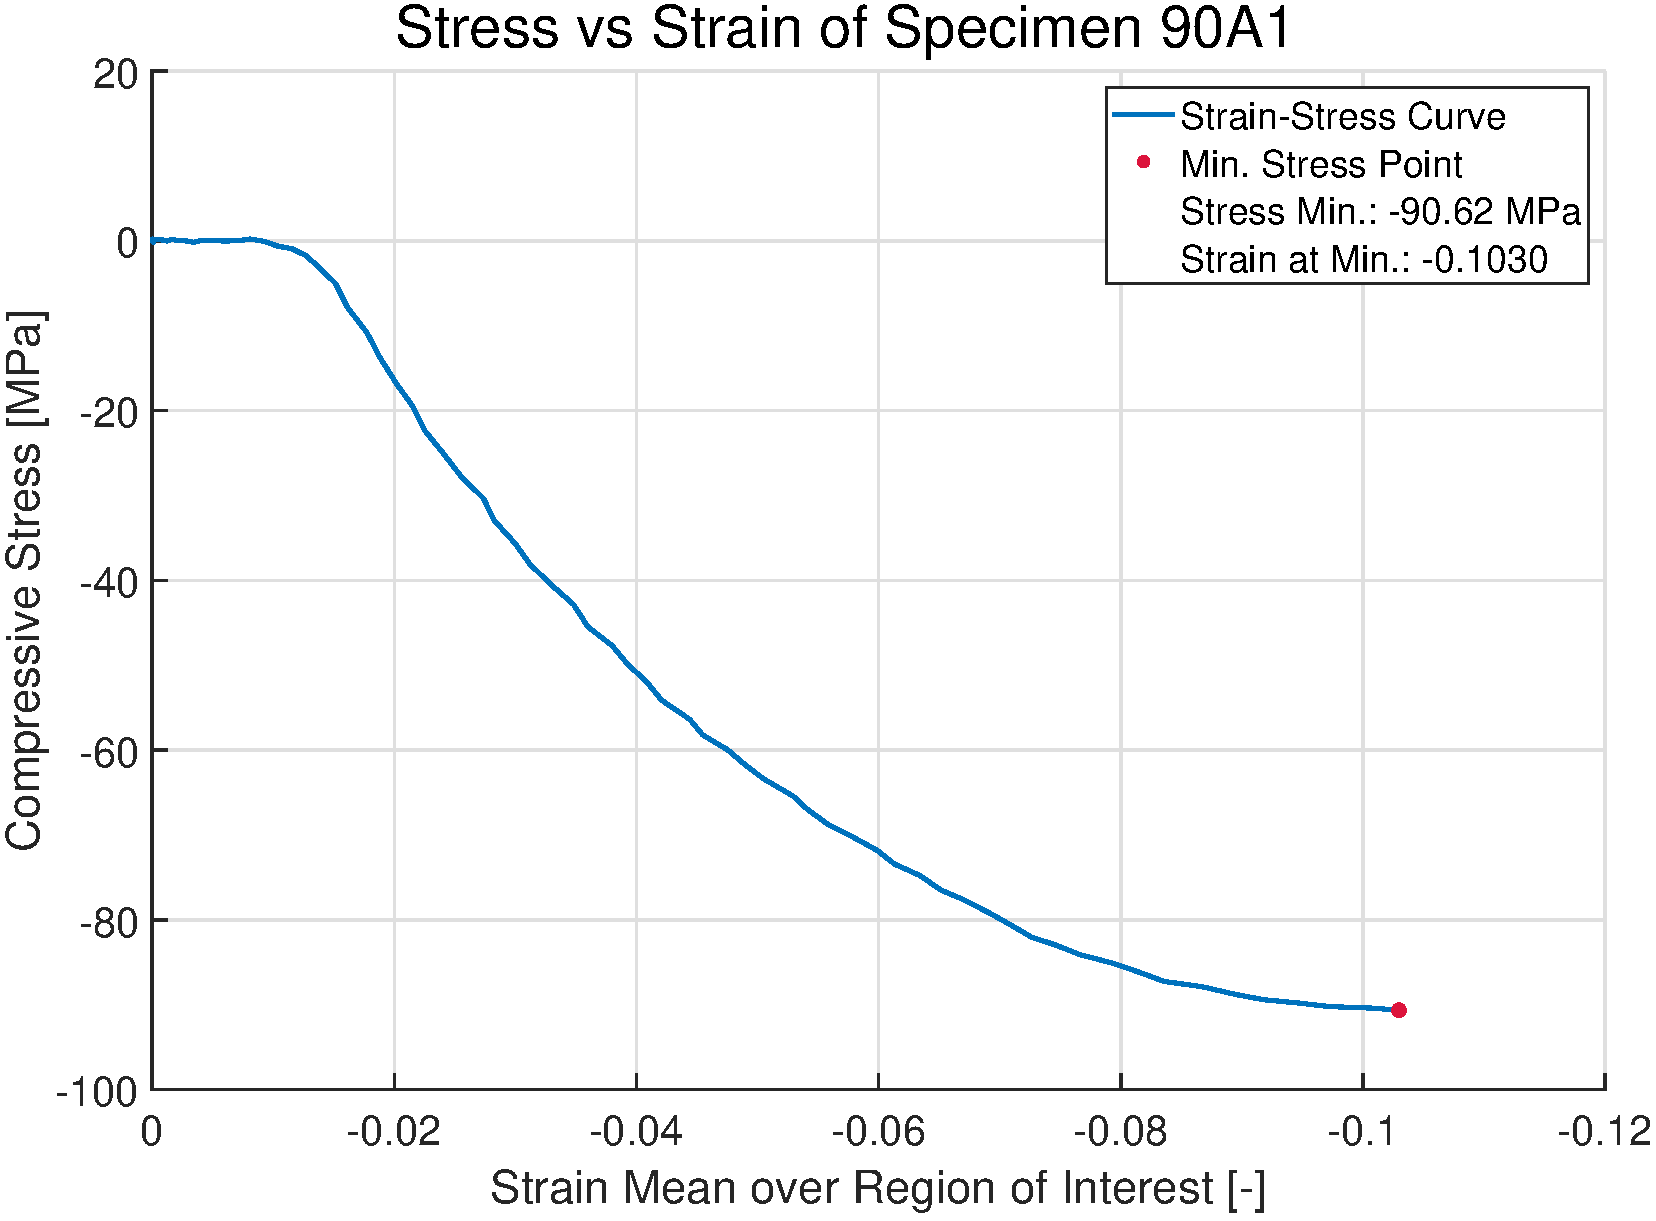
\includegraphics[scale=0.4]{\imgpath/\currfilebase/90A1_Stress_over_Strain}
    \caption{Stress over strain curve of experiment 90A1}
    \label{fig:90A1_Stress_over_Strain}
\end{figure}

\section{Absolute Compressive Stress at Failure}
\label{sec:abs_comp_stress}

The absolute compressive stress at Failure is the stress at peak load of the specimen. For the tested specimens, this corresponds to the point where the ultimate failure occurred. The stress is estimated by deviding the peak compressive force by the mean cross-section of the specimen at zero load\footnote{As depicted in \autoref{subsec:spec_dim}}:
\begin{align*}
    \tau_c &= \max\bqty{\frac{\abs{F_{c}}}{S}}, &S &= \frac{1}{3}\sum\limits_{i=2}^4 w_i\cdot t_i
\end{align*}
where $\tau_c$ is the absolute compressive stress at failure, $F_c$ the compressive force measured by the fatigue test system, $S$ the mean cross section of the specimen and $w_i$, $t_i$ the width and thickness of said specimen, measured at position $i$.

\newcommand{\visfeat}[1]{%
    \raisebox{-0.5ex}{%
        
\includegraphics[page=#1,scale=0.2]{\imgpath/\currfilebase/visual_features}}
}

The specimens were grouped into four different main failure categories based on the visual features of the tested specimen:
\begin{itemize}
    \item[\visfeat{1}] Failed in fixture first -- The failure occured in fixture where one is not able to record it by the CCD setup.
    \item[\visfeat{2}] Failed near fixture -- The failure propagated from fixture into FOI.
    \item[\visfeat{3}] Debonding at top end -- Debonding at the top end occured due to the specimen stiffness.
    \item[\visfeat{4}] Failure location in FOI -- The failure occurred in the FOI. This is the desired case for local strain analysis.
\end{itemize}
Furthermore, the crack line was categorized into 4 different types:
\begin{itemize}
    \item[\visfeat{5}] Failure perpendicular to fibre direction -- The crack line is perpendicular to the fibre direction.
    \item[\visfeat{6}] Interlaminar failure -- The crack line is in fibre direction or debonding occurred.
    \item[\visfeat{7}] Zigzag failure -- The crack line is both in and perpendicular to the fibre direction.
    \item[\visfeat{8}] 3-fold failure -- The fixed FOI cracked in fibre direction at 3 parallel lines. Specimens with failure of this type are split up into 4 parts.
\end{itemize}

\begin{figure}[!ht]
    \centering
    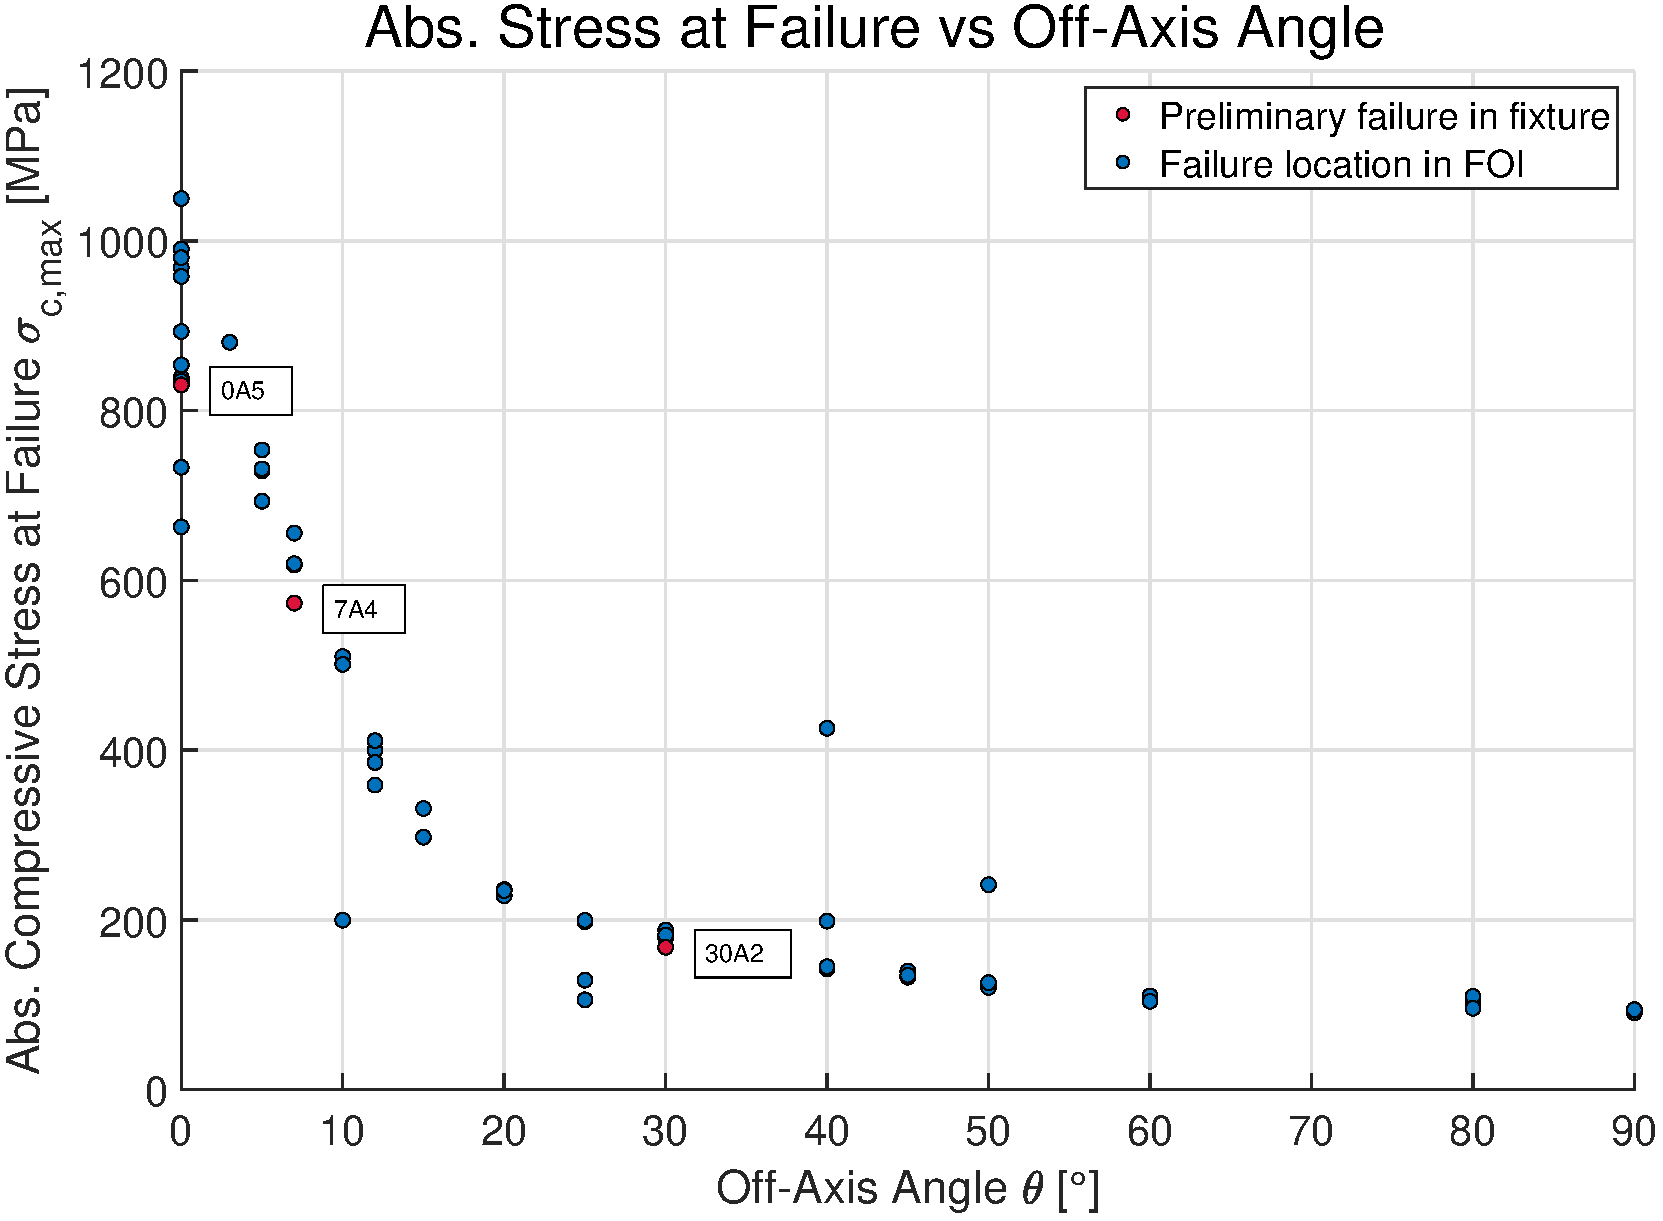
\includegraphics[scale=0.4]{\imgpath/\currfilebase/Strength_OffAngle_1.pdf}
    \caption{Abs. compressive stress at failure over off axis angle, failed in fixture}
    \label{fig:strength_offAngle_1}
\end{figure}
\begin{figure}[!ht]
    \centering
    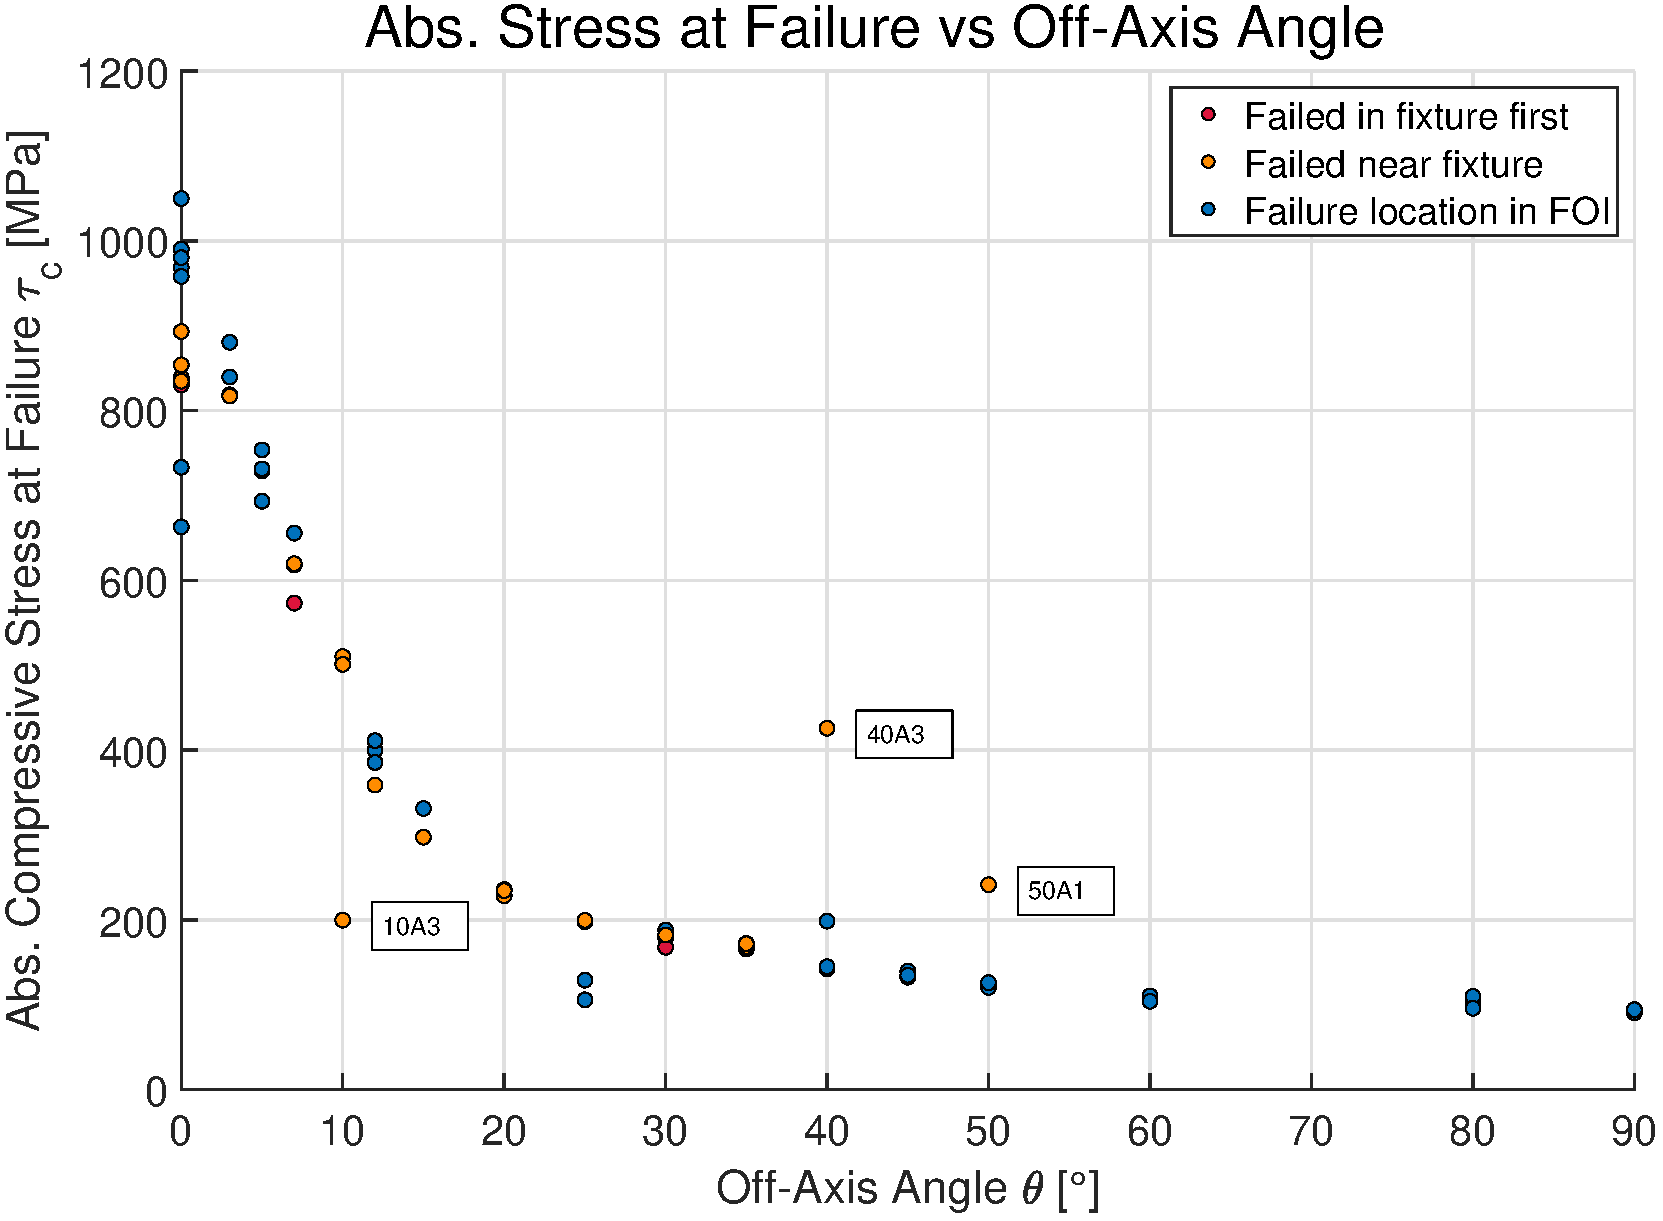
\includegraphics[scale=0.4]{\imgpath/\currfilebase/Strength_OffAngle_2.pdf}
    \caption{Abs. compressive stress at failure over off axis angle, failed near fixture}
    \label{fig:strength_offAngle_2}
\end{figure}
\begin{figure}[!ht]
    \centering
    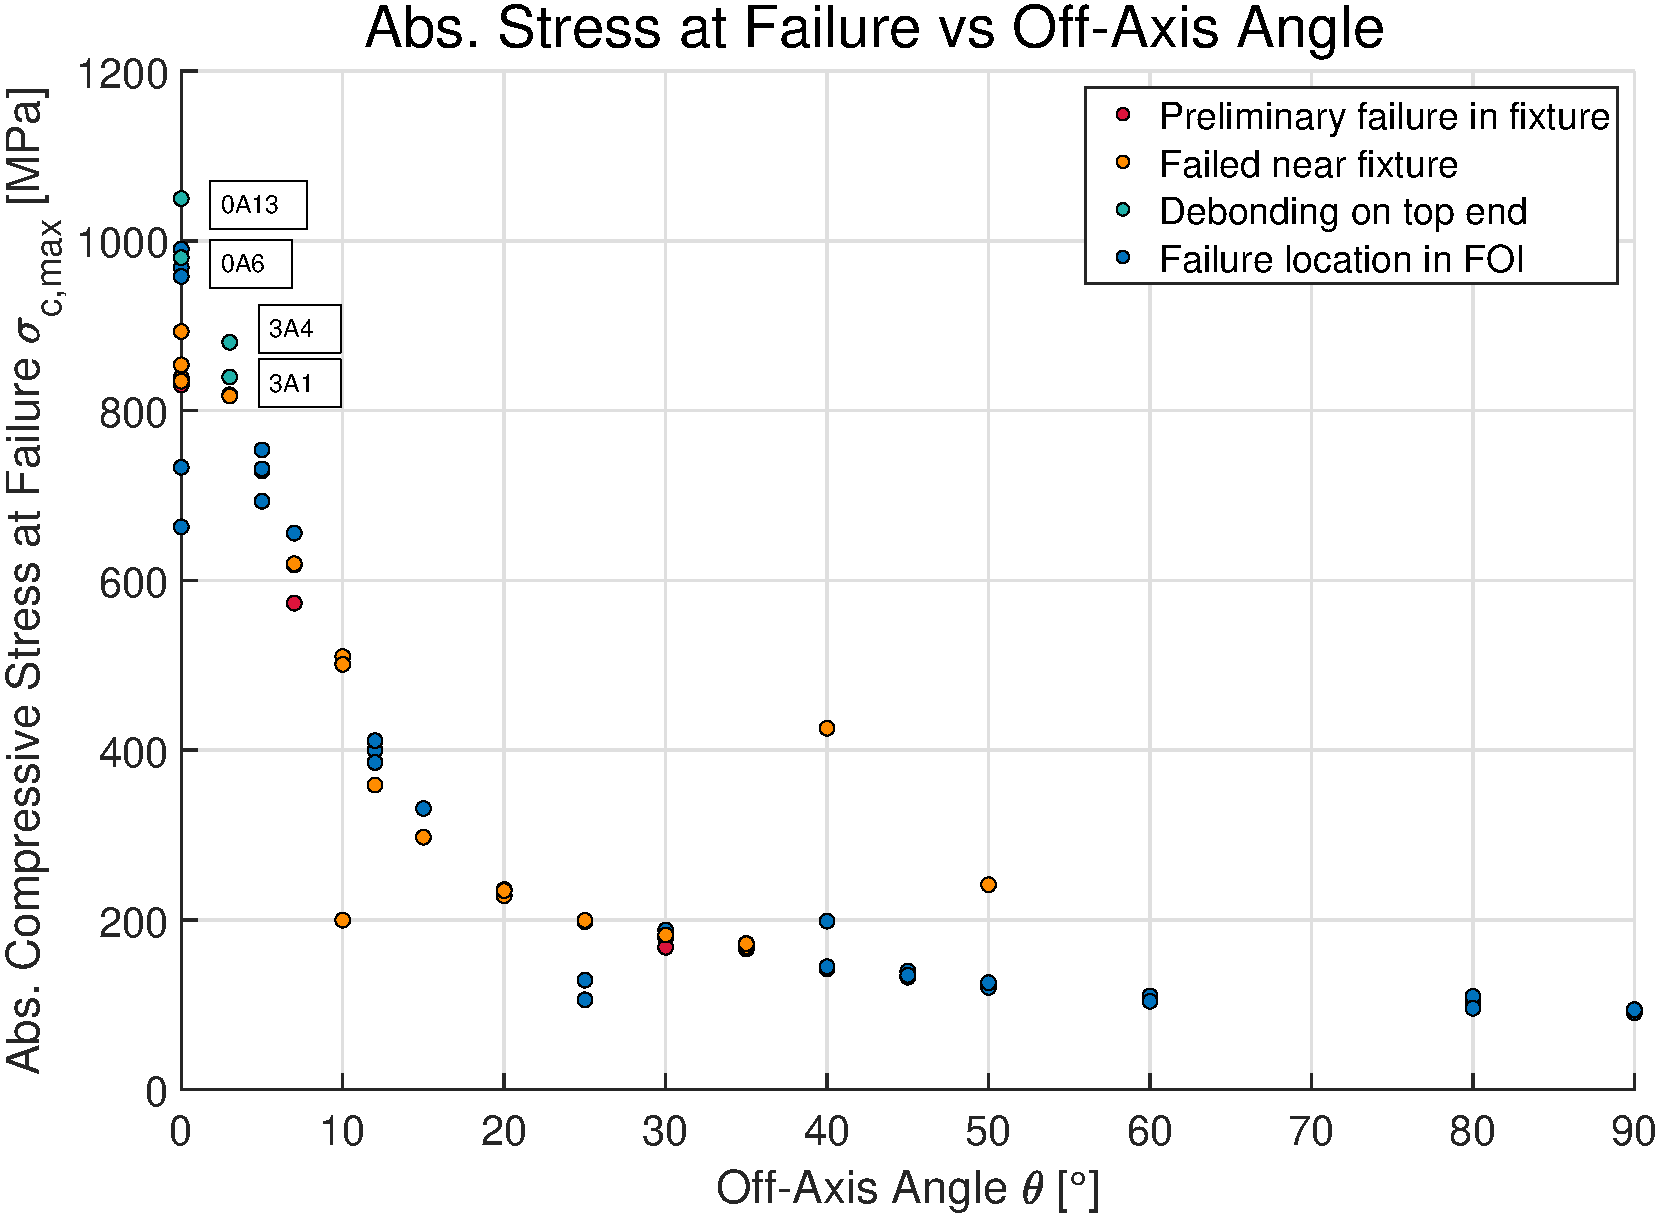
\includegraphics[scale=0.4]{\imgpath/\currfilebase/Strength_OffAngle_3.pdf}
    \caption{Abs. compressive stress at failure over off axis angle, debonding on top end}
    \label{fig:strength_offAngle_3}
\end{figure}
\begin{figure}[!ht]
    \centering
    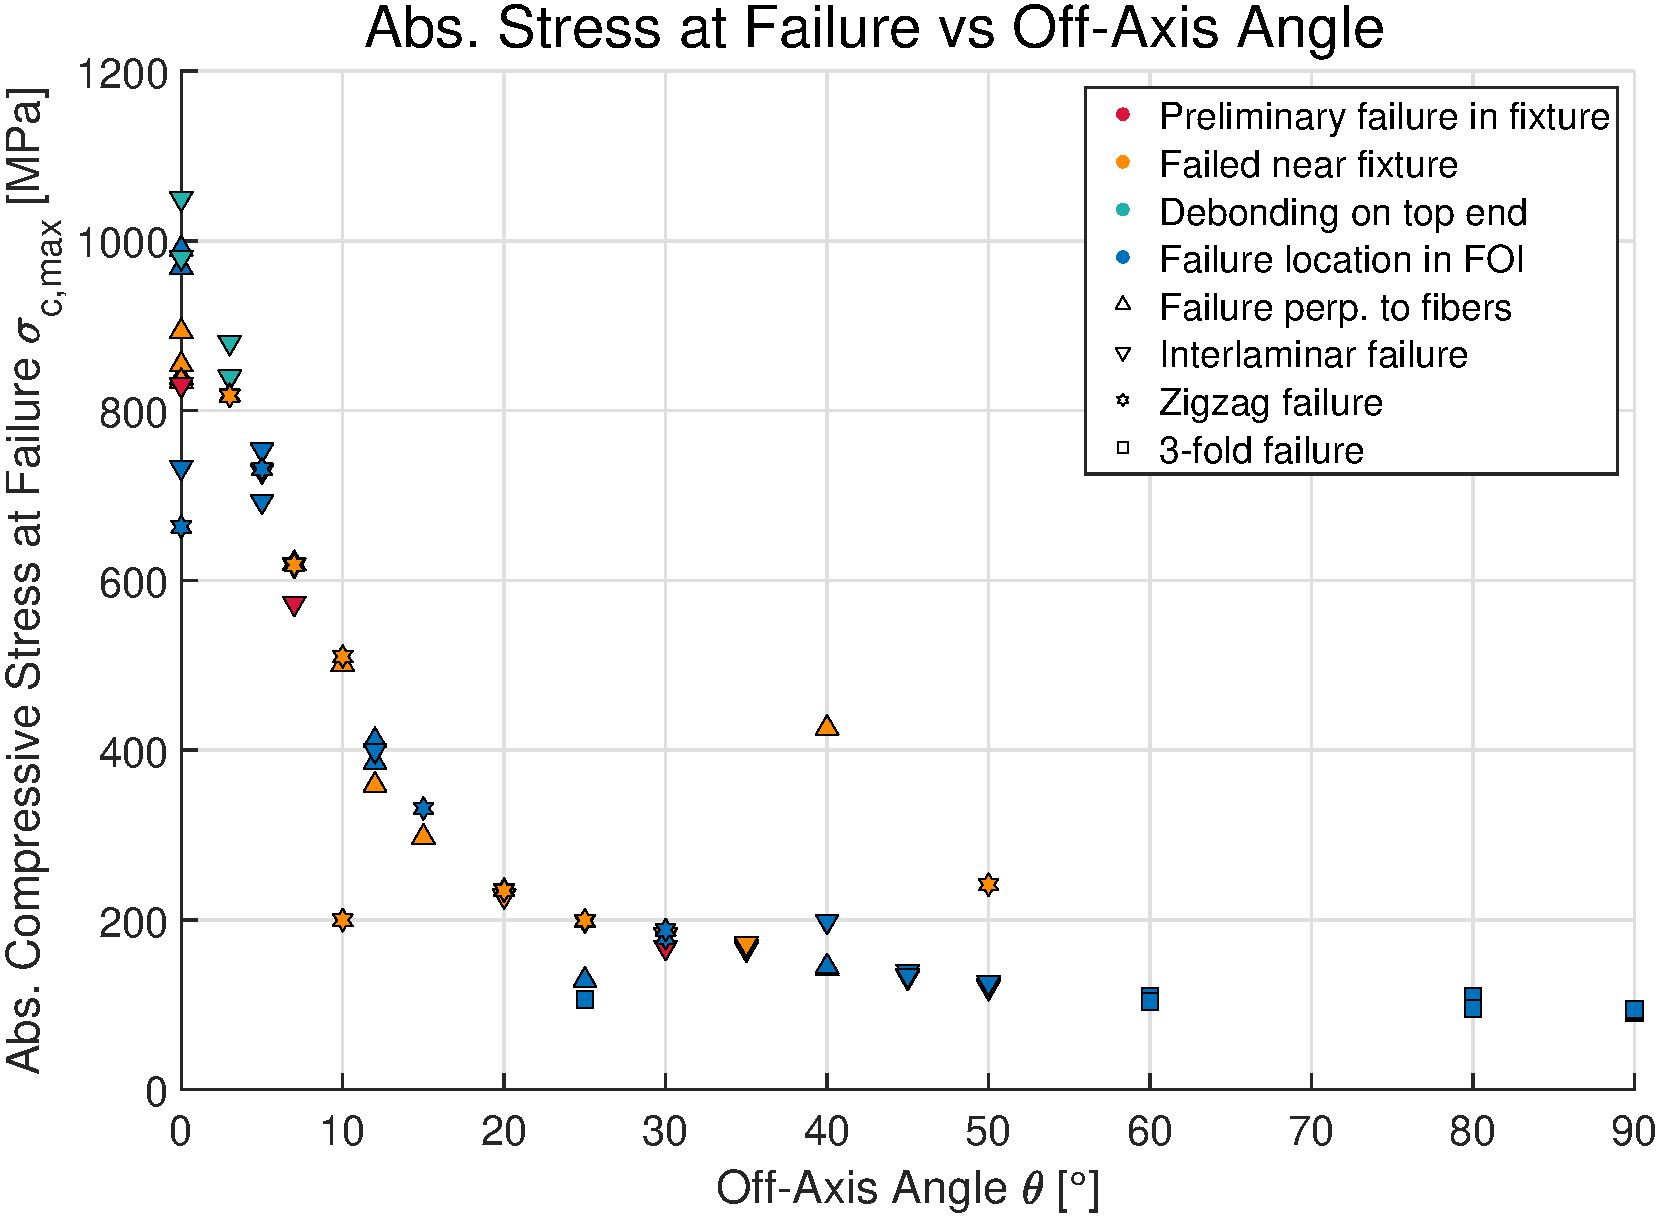
\includegraphics[scale=0.4]{\imgpath/\currfilebase/Strength_OffAngle_4.pdf}
    \caption{Abs. compressive stress at failure over off axis angle, categorized crack lines}
    \label{fig:strength_offAngle_4}
\end{figure}

\section{Discussion}
\label{sec:discussion}

\subsection*{Stress over Strain Curves}

The maximum stresses reached in testing were $\SI{20}{\percent}$ below the the manufacturers' specification. The  

\subsection*{Absolute Compressive Stress at Failure}

The absolute compressive stress at failure for the different off-axis angles show the expected pattern of an exponential decline at small off axis angles and quasi-linear decline at high off-axis angles. This pattern supports the tendency of higher variance at lower off-axis angles due to its slope if one does not take outliers into account. Namely specimens 0A1, 0A2, 0A3, 0A4, 0A5, 0A7, 0A10, 10A3, 25A2, 25A4, 40A2, 40A3 and 50A1 oppose this claim. Where 40A3 and 50A1 are of special interest because they surpassed the compressive strengths of a multitude of lower off-axis angle specimens.

\begin{footnotesize}
\begin{longtable}{@{}lccccccccccccc}
\hline
\thead{Feature} & \thead{0A1} & \thead{0A2} & \thead{0A3} & \thead{0A4} & \thead{0A5} & \thead{0A7} & \thead{0A10} & \thead{10A3} & \thead{25A2} & \thead{25A4} & \thead{40A2} & \thead{40A3} & \thead{50A1}\\
\hline \endhead
Failure category & \visfeat{2} & \visfeat{2} & \visfeat{2} & \visfeat{2} & \visfeat{1} & \visfeat{4} & \visfeat{4} & \visfeat{2} & \visfeat{4} & \visfeat{4} & \visfeat{4} & \visfeat{2} & \visfeat{2}\\
Crack line & \visfeat{5} & \visfeat{5} & \visfeat{5} & \visfeat{5} & \visfeat{6} & \visfeat{6} & \visfeat{7} & \visfeat{7} & \visfeat{5} & \visfeat{8} & \visfeat{6} & \visfeat{5} & \visfeat{7}\\
\hline
\caption[Overwiew outliers]{Overview of outlier measurements -- Measurements that do not fit the expected pattern (steep slope at low off-axis angles vs. quasi-linear at high off-axis angles)}
\label{tab:oultier_specimens}
\end{longtable}
\end{footnotesize}

Form \autoref{tab:oultier_specimens} one derives that the relationship between the visual failure category and the crack line to the classification of the measurement as outlier is non-trivial. However they are partially coupled to the off-axis angle. When the specimen has a low off-axis angle and when it is tabbed, debonding at its top end is more likely to occur. On the other hand if the specimen has a high off-axis angle, it is more prone to a 3-fold failure in the FOI.

The absolute compressive stress tends to be higher when debonding at the top end occurs. No conclusions can be drawn with regards to the other failure categories and crack lines.

When comparing established failure criteria to the experimental results they are mostly conservative and fit most data points well, see \autoref{fig:strength_offAngle_5}.
\begin{figure}[!ht]
    \centering
    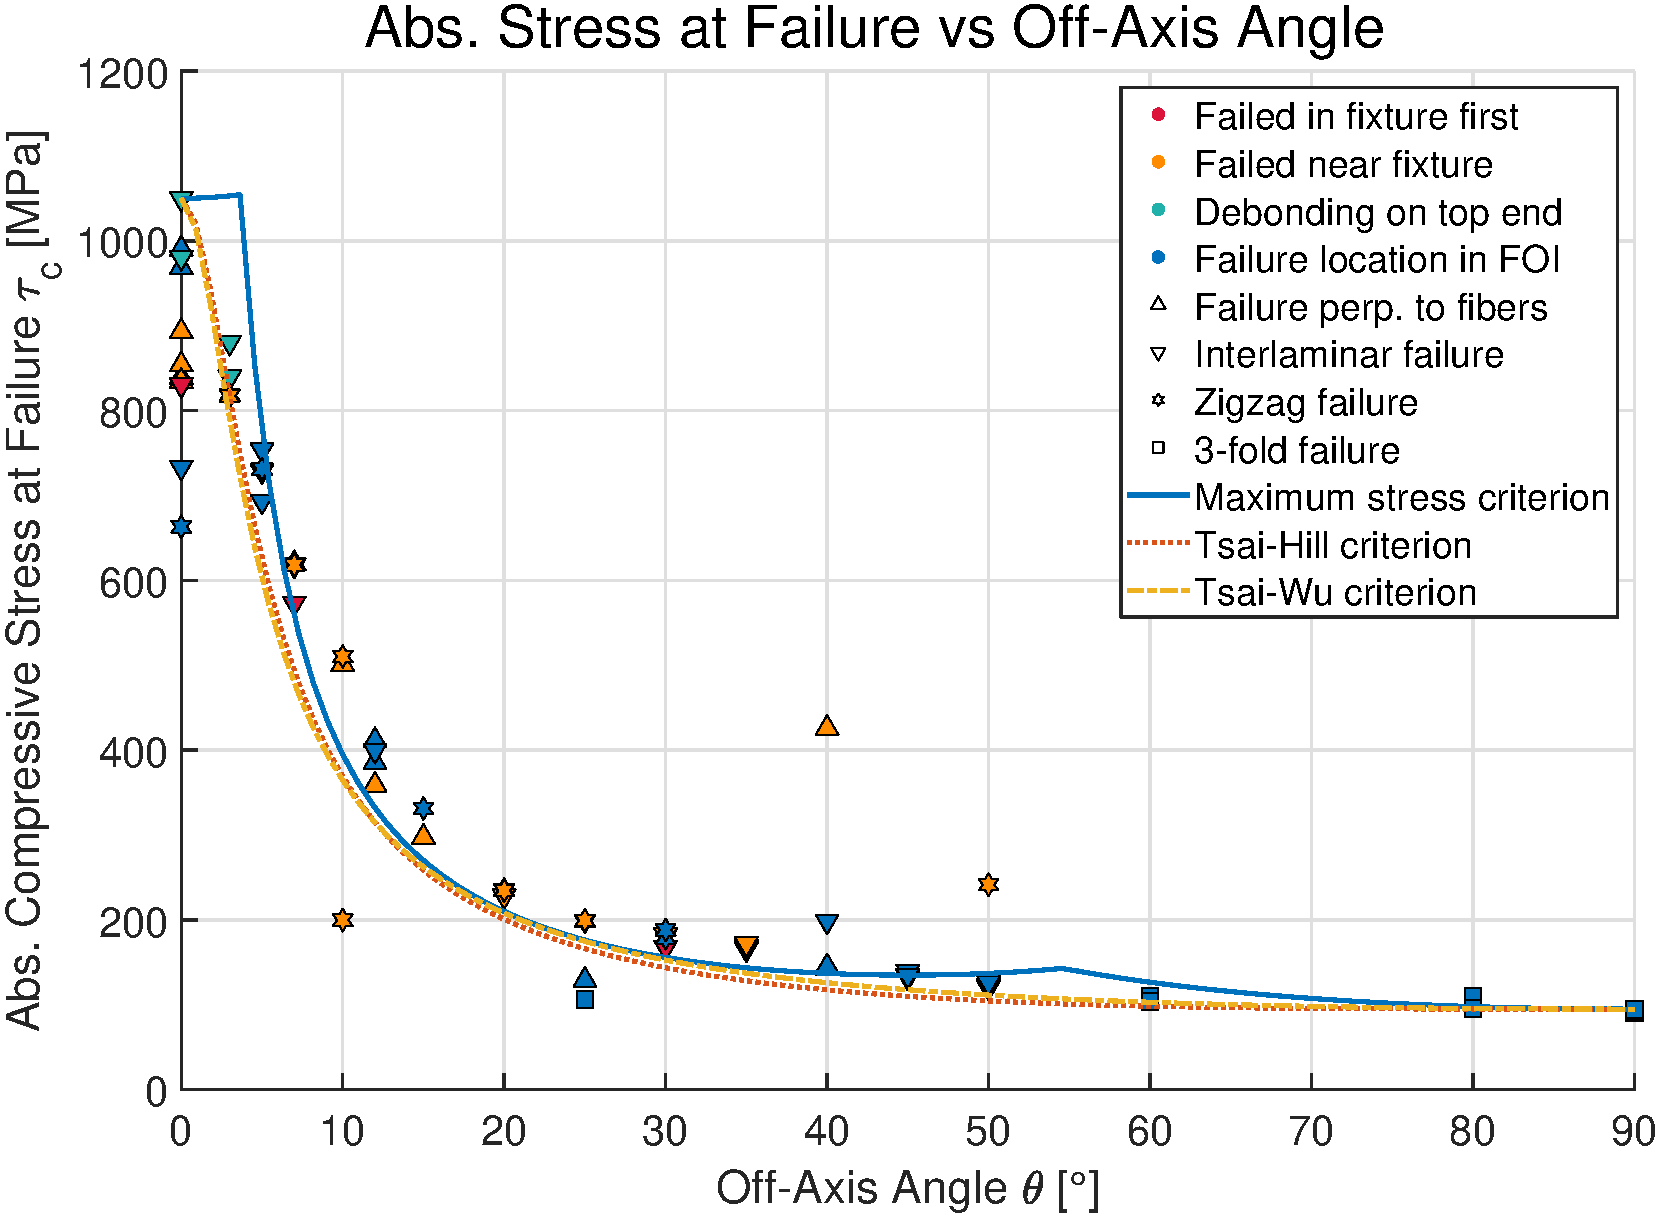
\includegraphics[scale=0.4]{\imgpath/\currfilebase/Strength_OffAngle_5.pdf}
    \caption{Abs. compressive stress at failure over off axis angle, failure criteria}
    \label{fig:strength_offAngle_5}
\end{figure}